\documentclass[11pt, fleqn]{article}

\usepackage{amsmath}
\usepackage{amsfonts}
\usepackage[margin=1in]{geometry} % To set the margin widths
\usepackage{graphicx}
\usepackage{listings}
\usepackage{multirow}
\usepackage{tabularx}
\usepackage{varioref}
\usepackage{cleveref}
\usepackage{siunitx}
\usepackage{subcaption}
\usepackage{titlesec}
\usepackage{bm}

\lstset{
  language=R,
  literate = {<-}{{$\gets$}}1 {~}{{$\sim$}}1
}

\sisetup{output-exponent-marker=\textsc{e}}

\titleformat{\section}[block]{\bfseries}{\thesection}{1em}{}

\setlength{\parskip}{12pt} % Sets a blank line in between paragraphs
\setlength\parindent{0pt} % Sets the indent for each paragraph to zero

\begin{document}

\title{Big Data: Homework 7}
\author{Will Clark \& Matthew DeLio \\ 41201-01}
\date{\today}
\maketitle

\section{Foreign Exchange Factor Modeling} \label{sec:intro}
% Discuss correlation amongst dimensions of fx. How does this relate to the applicability of factor modeling?
% From Wikipedia: Principal component analysis (PCA) is a statistical procedure that uses an orthogonal transformation to convert a set of observations of possibly correlated variables into a set of values of linearly uncorrelated variables called principal components. 
The data contained in \texttt{FXmonthly.csv} are monthly foreign exchange values between the us and various other countries.  To make them more comparable and useful for later analysis, we first transform them into a \%gain.  From here, we can discover how independent the currency movements are by running a simple correlation.  To visualize the correlation between the different currency we employ a heatmap (see \vref{fig:heatmap}).


\begin{figure}[!htb]
  \centering
  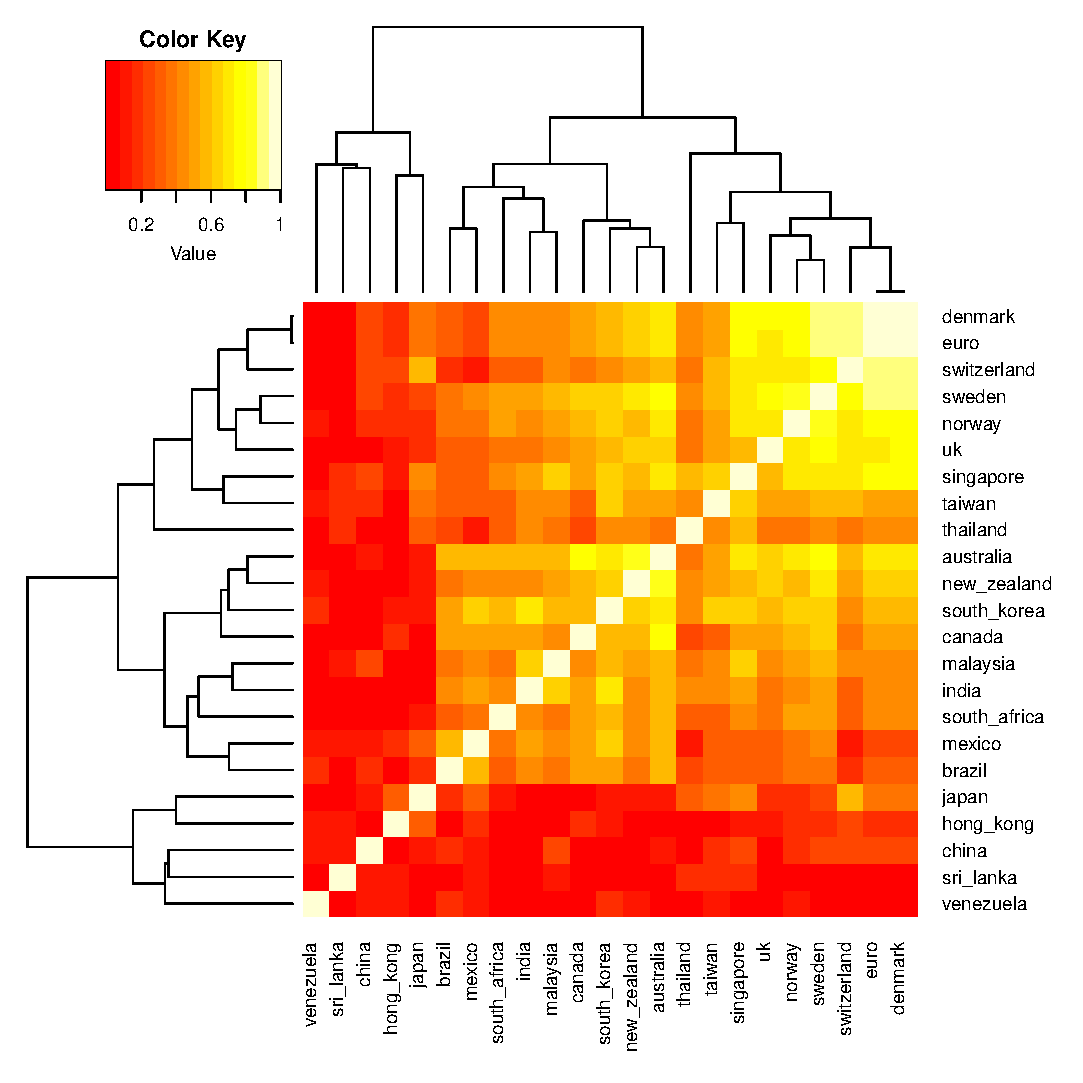
\includegraphics[scale=.7]{heatmap.eps}
  \caption{Foreign Exchange Correlation Heat-Map}
  \label{fig:heatmap}
\end{figure} 

\section{Principal Components Analysis} \label{sec:pca}
% Fit, plot, and interpret principal components.

At first glance, our data set of monthly foreign exchange rates seems to have a lot of noise and very little signal. The goal of principal components analysis is to see if there are any patterns connecting variables in our data set, and if there are, use these relationships to reduce the dimensionality of our data. To this end, we use \texttt{prcomp} to find the principal components of foreign exchange movements. For each observation $i$, which is a month of foreign exchange rates for 23 currencies, the method estimates:
\begin{equation}
E[x_i] = \varphi_i v_{i,1} + \varphi_2 v_{i,2} + ... + \varphi_k v_{i,k}
\end{equation}
We can now represent the data along the new set of dimensions $v_{i,j}$, which should reveal any latent patterns that were not observable when we were looking at the set of original dimensions $x_{i,j}$.

We can start by looking at the scree plot of our PCA, shown in Figure~\vref{fig:screeplot}. This shows us the sorted eigenvalues of the covariance matrix of the scaled data; the highest eigenvalue is the principal component that explains most of the variation in the data. The steep drop off after the first bar tells us that the first principal component explains a large degree of the variability in our data.

\begin{figure}[!htb]
  \centering
  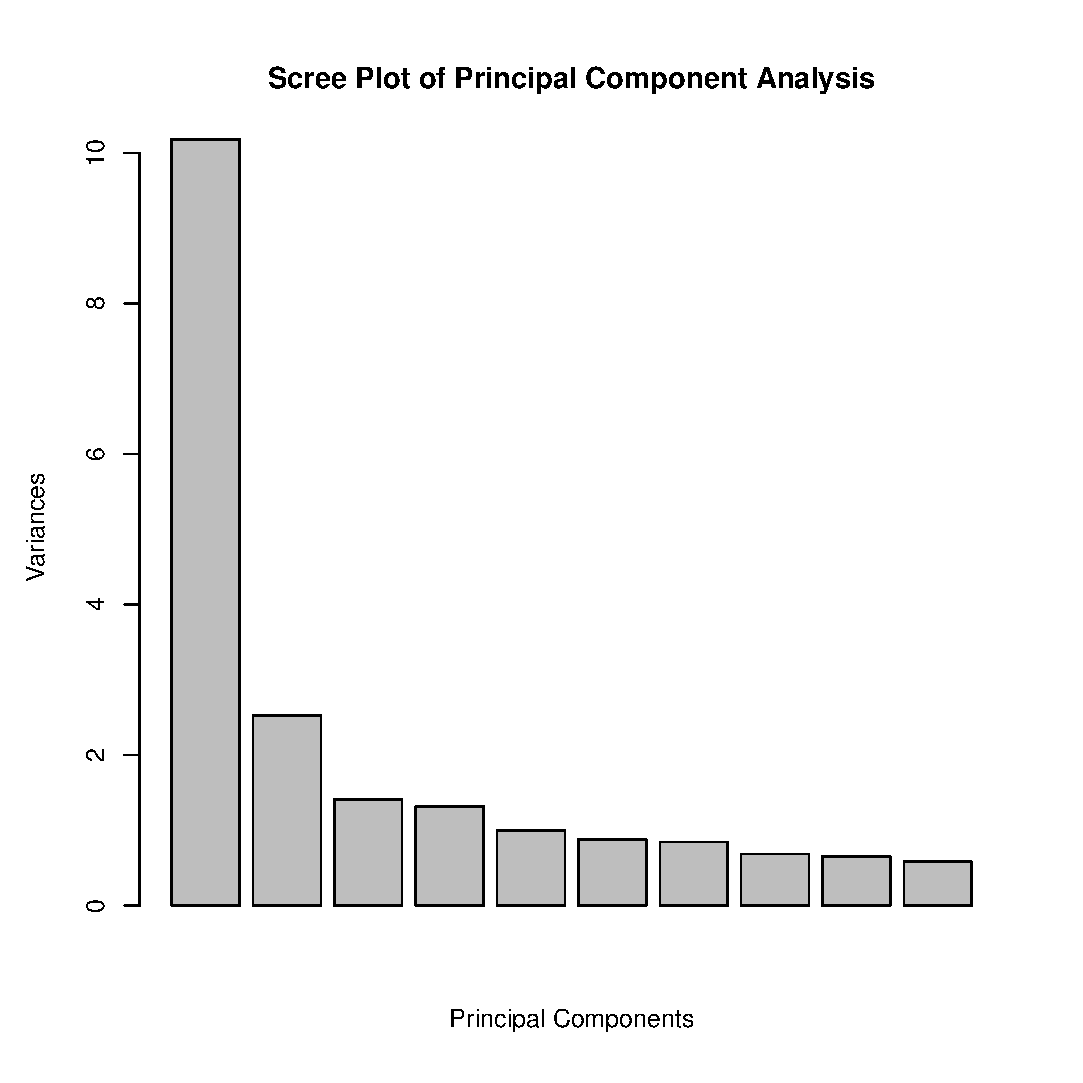
\includegraphics[scale=.5]{screeplot.eps}
  \caption{Foreign Exchange PCA Scree Plot}
  \label{fig:screeplot}
\end{figure} 

We can look at the rotations on the first principal component and see if there is any obvious interpretation. Figure~\vref{fig:pc1_pegs} shows the rotations of PC1 on each country; countries in red have floating exchange rates and countries in blue have fixed exchange rates (Venezuela, China, Hong Kong, and Sri Lanka). Given that all the pegged exchange rates are on one side and all the floating rates are on the other, we can tentatively conclude that the first principal component is really telling us about the fixed/floating divide. It makes sense that most of the variation in exchange rates would occur between those that are allowed to move freely and those that are not, and since PCA is supposed to find the latent sources of variation, it follows that this is the first dimension on which it chooses to sort the data.

\begin{figure}[!htb]
  \centering
  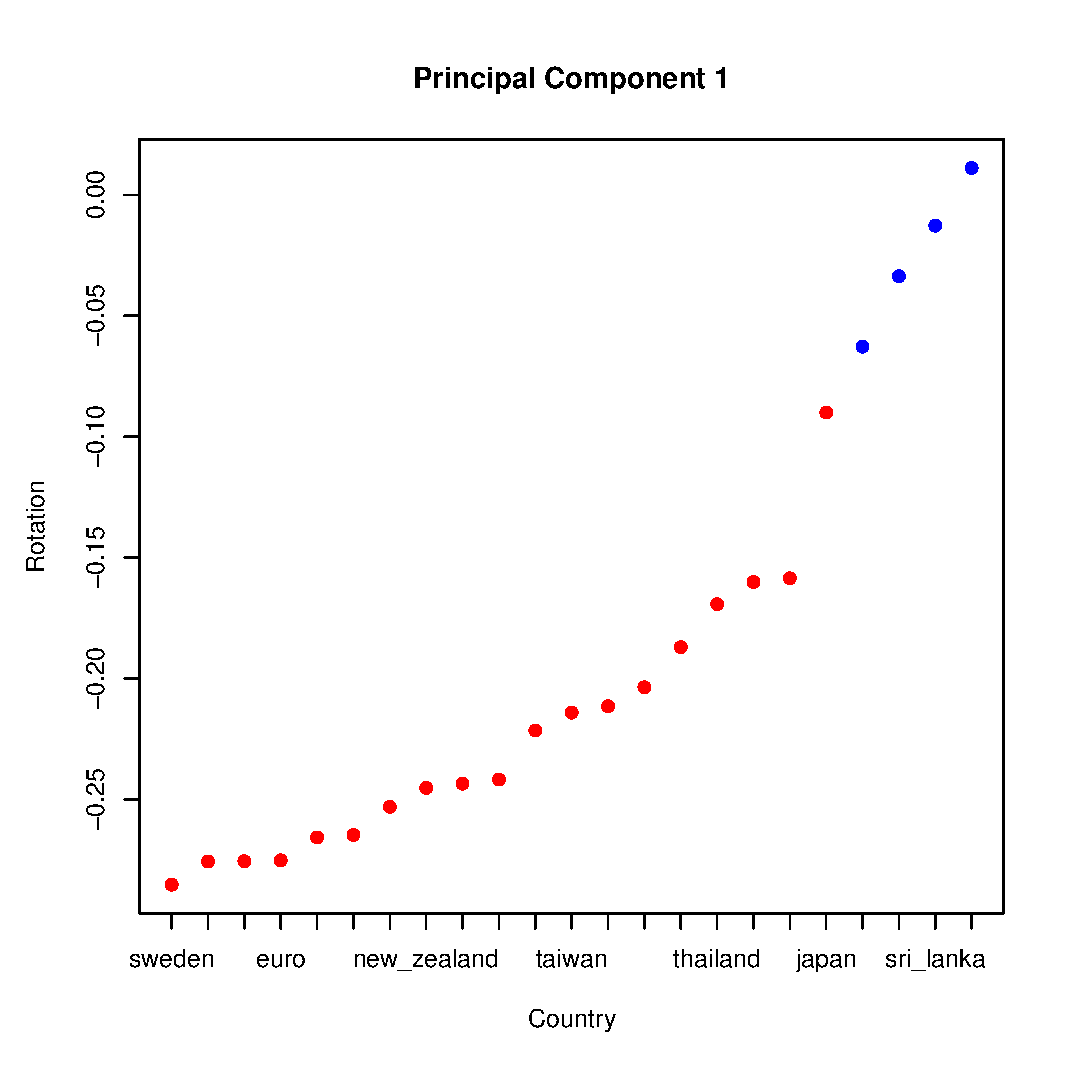
\includegraphics[scale=.5]{pc1_pegs.eps}
  \caption{Distribution of First Principal Component}
  \label{fig:pc1_pegs}
\end{figure} 

\section{S\&P 500 Returns on Currency Factors} \label{sec:sp500}

\section{Regression on All Covariates} \label{sec:regall}

\end{document}